\vfill


Tekst został zatwierdzony 31 maja 2019 roku przez Kongregację ds. Instytutów Życia Konsekrowanego i Stowarzyszeń Życia Apostolskiego.


\newpage




\section*{Preambuła}
\addcontentsline{toc}{part}{Preambuła}
\begin{enumerate}


% 1
\item Regnum Christi powstało jako eklezjalny ruch apostolski dążący do uobecniania Królestwa Chrystusa poprzez uświęcanie jego członków oraz poprzez osobistą i wspólnotową działalność apostolską zmierzającą ku temu, by Jezus Chrystus królował w sercach ludzi i społeczeństwie. 


% 2
\item Pierwsze świeckie grupy Regnum Christi powstały w 1968 roku dzięki zaproszeniu, działalności formacyjnej i kierowniczej duszpasterzy Legionistów Chrystusa oraz dzięki hojnemu przyjęciu i zapałowi samych świeckich. Ci mężczyźni i kobiety współdzielą jeden charyzmat, są pobudzani tym samym duchem i tą samą misją, przeżywając i realizując ją według swojego stanu życia. Świadomi własnego chrzcielnego powołania do świętości i do apostolstwa, czują się oni wezwani do bycia apostołami i do formowania apostołów - chrześcijańskich liderów w służbie Jezusowi Chrystusowi, Kościołowi i społeczeństwu. Ich zapał ewangelizacyjny objawia się także w dziełach apostolatu oraz w działalności na rzecz ogółu.


% 3
\item Od momentu pierwszego impulsu towarzyszącemu założeniu ruchu Regnum Christi zaczęły pojawiać się w nim takie formy konsekracji, w których świeccy kobiety i mężczyźni powierzają swe życie Bogu, aby móc swobodnie i całkowicie podążać za Chrystusem poprzez potwierdzone świętym węzłem przyjęcie ewangelicznych cnót ubóstwa, czystości i posłuszeństwa. Grupy te stopniowo nabierały dojrzałości instytucyjnej i ewangelizacyjnego zasięgu, znacząco przyczyniając się do istoty Regnum Christi.


% 4
\item Duchowa rodzina Regnum Christi złożona jest dzisiaj ze świeckich, zarówno stanu wolnego, jak i zamężnych czy żonatych, świeckich konsekrowanych kobiet i mężczyzn, seminarzystów, diakonów i księży diecezjalnych, kleryków i księży Legionistów Chrystusa. Każdy z nich na swój sposób przeżywa swoje powołanie, będąc jednocześnie członkiem jednego ciała (1 List do Koryntian 12, 12-29) i oddając się jednej wspólnej misji.


% 5
\item Na przestrzeni dziesięcioleci zarząd Regnum Christi był złączony i utożsamiony z zarządem Legionu Chrystusa, co zostało potwierdzone w Statutach Regnum Christi zatwierdzonych w 2004 roku przez Stolicę Apostolską. W 2012 roku delegat papieski, kardynał Velasio De Paolis CS, nadał konsekrowanym kobietom i mężczyznom autonomię organizacji rządów i życia wewnętrznego. W 2013 roku zatwierdził Statuty ich własnych stowarzyszeń wiernych, pozostawiając otwartą kwestię ich całkowitego zatwierdzenia kanonicznego oraz definicji prawnej na temat ich przynależności do Regnum Christi. Kolejny, decydujący krok nadszedł 25 listopada 2018 roku w uroczystość Jezusa Chrystusa, Króla Wszechświata, kiedy to oba stowarzyszenia zostały podniesione do rangi stowarzyszeń życia apostolskiego opartych na prawie pontyfikalnym.


% 6
\item W latach 2014-2018 z pomocą asystenta papieskiego, ojca Gianfranco Ghirlanda SJ, dokonywał się proces rozpoznania i analizy elementów składowych Regnum Christi w celu znalezienia takiej struktury kanonicznej, która wyrażałaby duchową jedność i współpracę apostolską wszystkich osób, która promowałaby tożsamość i prawowitą autonomię każdego konsekrowanego podmiotu, i która pozwalałaby innym wiernym Regnum Christi przynależeć do tego samego ciała apostolskiego w sposób kanonicznie potwierdzony. Aby osiągnąć te cele, Zgromadzenie Księży Legionistów Chrystusa, Wspólnota Życia Apostolskiego „Konsekrowane Regnum Christi” oraz Wspólnota Życia Apostolskiego „Świeccy Konsekrowani Regnum Christi” łączą się ze sobą poprzez Federację Regnum Christi, do której również mogą indywidualnie przyłączyć się inni wierni podzielający tego samego ducha i tę samą misję. Natura, struktura, cele i działalność Federacji zostały określone w niniejszych Statutach.


% 7
\item Nowa postać kanoniczna Regnum Christi jest, poprzez strukturę Federacji, owocem ścieżki odnowy i dojrzałości w Kościele, ścieżki którą kroczą wszyscy jej członkowie. Regnum Christi dziękuje Bogu i Kościołowi za ten krok naprzód, który pozwala lepiej wyrazić jedność i współodpowiedzialność wszystkich członków, ponadto stanowi dla nich impuls w misji uobecniania Królestwa Chrystusa w świecie.


\end{enumerate}




\begin{figure}
\addcontentsline{toc}{part}{Dekret powołania Federacji}
\begin{center}
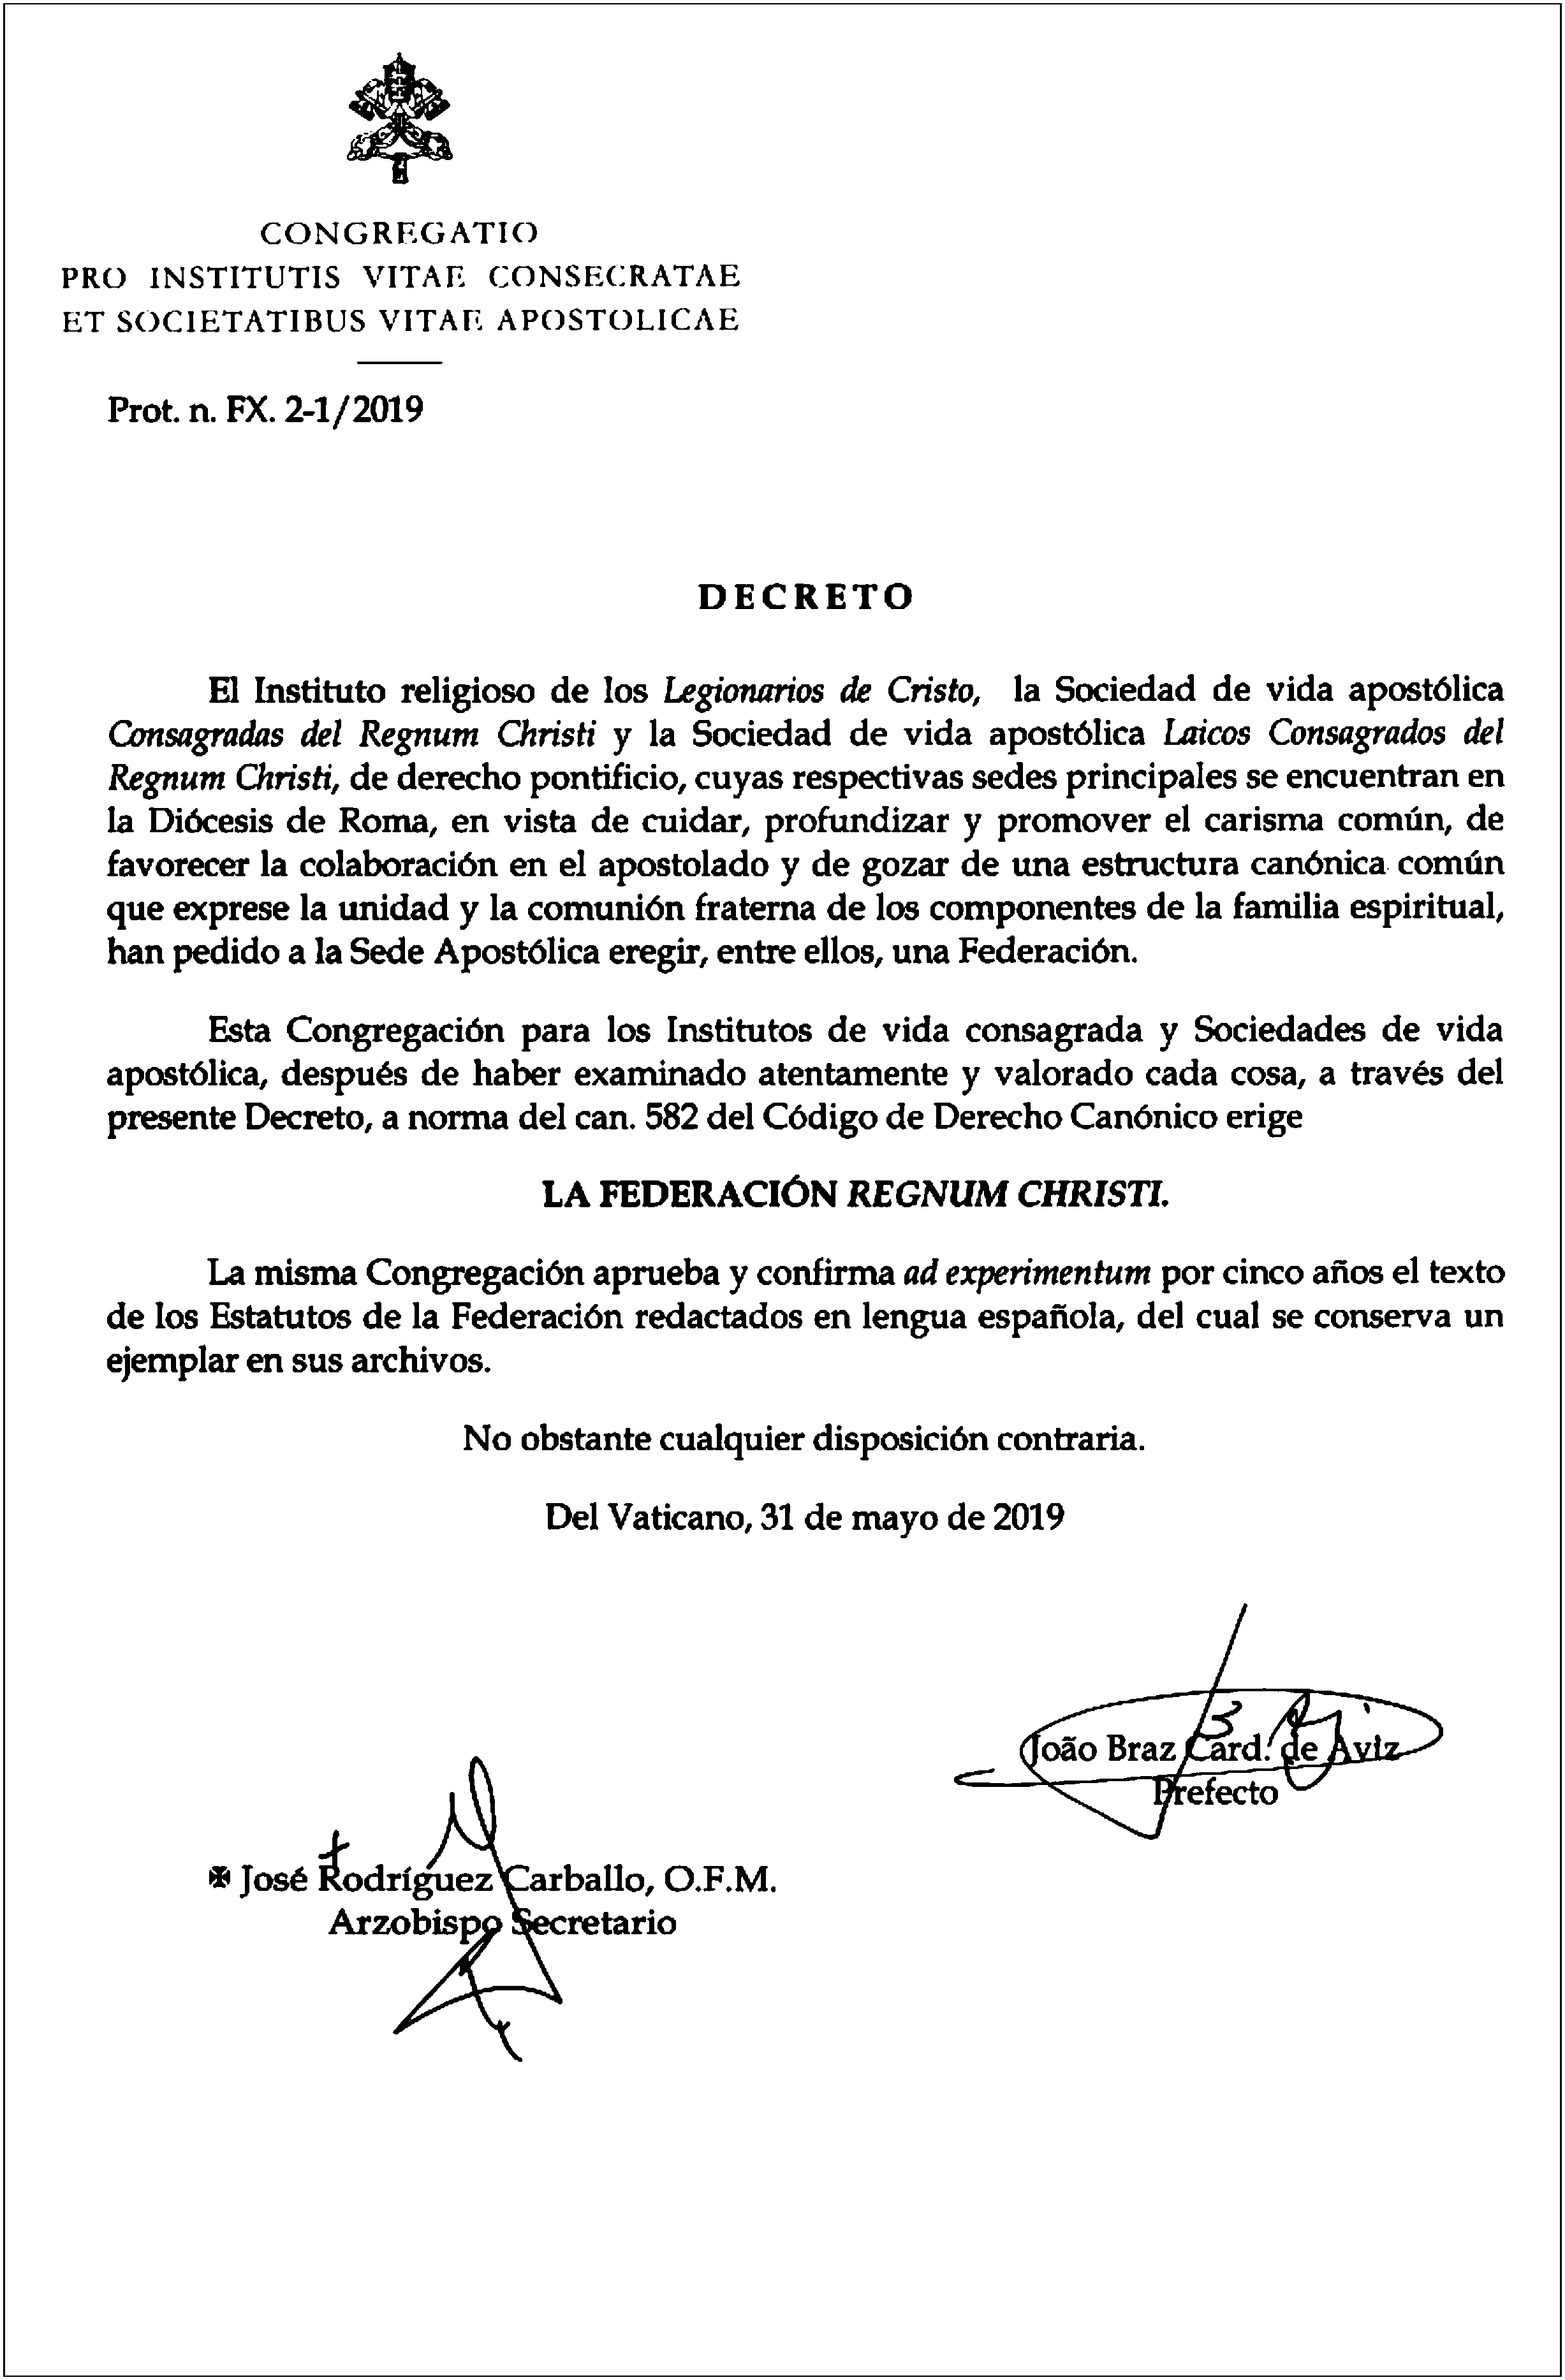
\includegraphics[height=\textheight]{dekret-powolanie-federacji-rc}
\end{center}
\end{figure}






\begin{figure}
\begin{framed}
\begin{footnotesize}






\begin{tabular}{c}
{\em logo} \vspace{.5em} \\
CONGREGATIO\\
PRO INSTITUTIS VITAE CONSECRATAE\\
ET SOCIETATIBUS VITAE APOSTOLICAE 


\end{tabular}




\vspace{1em}
Protokół nr FX. 2-1/2019






\begin{center}DEKRET\end{center}


Religijny Instytut Legionistów Chrystusa, Wspólnota Życia Apostolskiego Konsekrowane Regnum Christi oraz Wspólnota Życia Apostolskiego Świeccy Konsekrowani Regnum Christi, uznane na prawie pontyfikalnym, z siedzibą w Diecezji Rzymskiej, dążąc do zapewnienia odpowiedniej opieki, do pogłębiania, promowania wspólnego charyzmatu, do wzmacniania współpracy w ramach apostolatu oraz do tworzenia wspólnej struktury kanonicznej, która mogłaby wyrazić jedność braterską wszystkich składowych tej duchowej rodziny, złożyły wniosek do Stolicy Apostolskiej z prośbą o powołanie między nimi Federacji.


Kongregacja ds. Instytutów Życia Konsekrowanego i Stowarzyszeń Życia Apostolskiego, po uprzednim uważnym przeanalizowaniu i rozważeniu wszystkich czynników, za pośrednictwem niniejszego Dekretu, na mocy kanonu 582 Kodeksu prawa kanonicznego, powołuje:


\begin{center}FEDERACJĘ REGNUM CHRISTI\end{center}


Kongregacja jednocześnie zatwierdza kształt Statutów Federacji, oryginalnie zredagowanych w języku hiszpańskim i zdeponowanych w archiwum Kongregacji, na próbny okres {\em ad experimentum} pięciu lat. 


\begin{center}
Nie naruszając wszelkich przeciwnych postanowień

podpisano w Watykanie, 31 maja 2019 roku.
\end{center}
 
\hfill\begin{tabular}{c}
{\em podpis} \\
João Braz Kard. de Aviz \\
Prefekt
\end {tabular}


\begin{tabular}{c}
{\em podpis} \\
José Rodríguez Carballo, OFM\\
Arcybiskup Sekretarz 
\end{tabular}
 
\end{footnotesize}
\end{framed}
\end{figure}






% Część pierwsza 
\part{Tożsamość, członkowie i działalność\\Federacji Regnum Christi}


% Rozdział 1
\chapter{Natura, struktura i cele}


\ssec{Natura i struktura instytucjonalna}


\lett{1} \S{}1. Federacja Regnum Christi składa się ze Zgromadzenia Księży Legionistów Chrystusa, Wspólnoty Życia Apostolskiego „Konsekrowane Regnum Christi” oraz Wspólnoty Życia Apostolskiego „Świeccy Konsekrowani Regnum Christi”.


\S{}2. Instytucje te, złączone w federację, zachowują swoją tożsamość, cele i prawowitą autonomię w rozumieniu Prawa Kanonicznego oraz odpowiednich konstytucji.


\S{}3. Federacja Regnum Christi posiada osobowość prawną. 


\ssec{Stowarzyszeni wierni}


\lett{2} Do Federacji mogą indywidualnie dołączyć inni wierni, dopuszczeni przez dyrektorów sekcji, zgodnie z postanowieniami przepisów własnych, które zostały zatwierdzone przez Konwencję Generalną Federacji, a mianowicie:


\begin{enumerate}


% 1
\item świeccy wierni, którzy nie podjęli zobowiązań ewangelicznych potwierdzonych świętym węzłem, i którzy osobiście przyjęli wezwanie do pełnego przeżywania swoich zobowiązań chrzcielnych w doczesnej rzeczywistości według ducha i misji, którymi inspiruje się Federacja;


% 2
\item kapłani, diakoni i seminarzyści diecezjalni.


\end{enumerate}
 
\ssec{Regnum Christi}


\lett{3} Zgromadzenie Księży Legionistów Chrystusa, Wspólnota Życia Apostolskiego „Konsekrowane Regnum Christi” oraz Wspólnota Życia Apostolskiego „Świeccy Konsekrowani Regnum Christi”, ich członkowie i wierni stowarzyszeni w Federacji indywidualnie – należą oni do Regnum Christi – jednej rodziny duchowej i jednego ciała apostolskiego.


\ssec{Cele Federacji}


\lett{4} Oto charakterystyczne  cele Federacji:


\begin{enumerate}


%1
\item dostarczenie struktury kanonicznej, która wyrazi jedność charyzmatu wszystkich elementów Federacji przy jednoczesnym uszanowaniu tożsamości każdego z nich z osobna;


%2
\item doglądanie, pogłębianie i promowanie wspólnego dziedzictwa charyzmatu;


%3
\item stymulowanie rozwoju wspólnej misji na rzecz Kościoła i społeczeństwa;


%4
\item promowanie postawy współpracy w działaniach apostolskich stowarzyszonych instytucji;


%5 
\item kierowanie działalnością apostolską Federacji;


%6
\item promowanie idei wspólnoty i zapewnianie poczucia jedności pomiędzy stowarzyszonymi instytucjami oraz wiernymi stowarzyszonymi w Federacji;


%7
\item regulowanie i sprawowanie kontroli nad uczestnictwem stowarzyszonych wiernych oraz troska o ich proces formacji;


%8
\item promowanie rozwoju i wzrostu powołania wśród stowarzyszonych instytucji oraz stowarzyszonych wiernych;


%9
\item doraźna pomoc instytucjom stowarzyszonym w Federacji oraz wspieranie idei solidarności pomiędzy regionami, sekcjami i dziełami apostolskimi, na miarę aktualnych okoliczności i potrzeb.


\end{enumerate}
 
\ssec{Wkład własny każdej stowarzyszonej instytucji oraz stowarzyszonych wiernych}


\lett{5} Dla wspólnego dobra i rozwoju:


\begin{enumerate}


%1
\item Członkowie Wspólnoty Życia Apostolskiego „Konsekrowane Regnum Christi”, ze względu na swoją kobiecą tożsamość, wnoszą do Federacji dar świeckiego poświęcenia się poprzez całkowite i wyłączne powierzenie się miłości Chrystusa, będąc znakiem Jego Królestwa w doczesnej rzeczywistości, promując i troszcząc się o jedność, wychodząc na spotkanie z osobami w konkretnych sytuacjach życia oraz podejmując akcje, które przyczyniają się do ustanowienia Królestwa Chrystusa.


%2
\item Członkowie Wspólnoty Życia Apostolskiego „Świeccy konsekrowani Regnum Christi” wnoszą do Federacji dar własnego świeckiego poświęcenia się  poprzez prorocze świadectwo o byciu w świecie bez przynależności do świata, poprzez ewangelizację doczesnej rzeczywistości, swoją dyspozycyjność, miłość braterską, osobiste predyspozycje, radość w posłudze Regnum Christi, Kościołowi i ludziom; a także poprzez promocję jedności braterskiej i modlitwę. Przeżywają oni tajemnicę Chrystusa poświęconego Ojcu, bliskiego swoim braciom-ludziom, traktowanego jak zwykłego człowieka spośród ludu, a swoim życiem, pracą i słowem głoszą wszystkim ludziom Jego Królestwo.


%3
\item Legioniści Chrystusa, z uwagi na swoją konsekrację zakonną, wnoszą do Federacji świadectwo oddania Jezusowi Chrystusowi oraz swoją całkowitą gotowość do realizowania wspólnej misji. Ze względu na swój status kapłanów uobecniają innym Chrystusa Kapłana i Dobrego Pasterza poprzez kaznodziejską posługę, udzielanie sakramentów oraz przewodnictwo duchowe. Razem ze wszystkimi biorą udział w integralnej formacji stowarzyszonych wiernych, w kierowaniu nimi oraz w procesie ich apostolskiego rozeznania, wspierając ich chrzcielne powołanie oraz predyspozycje do chrześcijańskiego przewodzenia innym. Powołują również niezbędne instytucje i podejmują działania, które w swoim zasięgu i natężeniu najbardziej mogą przyczynić się do ustanowienia Królestwa Chrystusa w społeczeństwie.


%4
\item Wierni stowarzyszeni wnoszą do Federacji swój świecki charakter i swoją działalność apostolską. Świeccy przedłużają obecność Chrystusa w świecie i dążą do ewangelicznej przemiany rzeczywistości doczesnej, zwłaszcza na polu życia rodzinnego, zawodowego i społecznego.


\end{enumerate}


% Rozdział 2
\chapter{Fundamenty Federacji Regnum Christi}


\section{Punkt 1. Fundamenty duchowe}


\ssec{Duchowe podwaliny}


\lett{6} Uważamy, że zamysłem Bożym jest, abyśmy jako Legioniści Chrystusa, Konsekrowane Regnum Christi, Świeccy Konsekrowani Regnum Christi i wierni stowarzyszeni żyli w prawdziwej wspólnocie i byli świadkami miłości Jezusa Chrystusa, która przejawia się w jedności  i miłości braterskiej jakie panują między nami. Wymienione instytucje, ich członkowie i wierni stowarzyszeni – współdzielimy duchowość i misję, które każdy przeżywa zgodnie ze swoją tożsamością i według swojego powołania, wyrażonych we własnych regułach. Ten duchowy fundament powinien inspirować i ukierunkowywać odpowiednie organy Federacji na poszczególnych stopniach i w przeróżnych okolicznościach czasu i miejsca.


\ssec{Najwyższy z celów}


\lett{7} Dążymy do oddawania chwały Bogu i uobecniania Królestwa Chrystusa w sercach ludzi i społeczeństwie dzięki osobistemu uświęceniu w okolicznościach życia, w jakich powołuje nas Bóg oraz poprzez indywidualne i wspólnotowe działania apostolskie.


\ssec{Nasza misja}
 
\lett{8} Wypełniając naszą misję staramy się uobecniać misterium Chrystusa, który wychodzi innym osobom na spotkanie, objawia im miłość swego Serca, gromadzi ich i formuje na apostołów, liderów chrześcijańskich, posyła i towarzyszy im we współpracy z Nim w ewangelizacji ludzi i całego społeczeństwa.


\ssec{Płodność apostolska}
 
\lett{9} {Ś}wiadomi tego, że Królestwo Chrystusa jest darem i nie można go zbudować wyłącznie ludzkim wysiłkiem, staramy się zawsze pozostawać w jedności z Chrystusem i z Jego Kościołem niczym latorośle wyrastające na krzewie winnym (por. J 15, 5). Jako naśladowcy i współpracownicy Chrystusa Apostoła wiemy, że modlitwa, udział w niesieniu krzyża, bezinteresowna posługa innym, zaufanie działaniu Jego łaski oraz świadectwo prawdziwie chrześcijańskiego życia muszą być priorytetem i towarzyszyć całej naszej działalności apostolskiej.
 
\ssec{Postawa ofiarności}
 
\lett{10} Osobiste doświadczenie miłości Chrystusa budzi w naszym sercu wewnętrzną potrzebę gorliwego oddania się Jemu i uobecniania Jego Królestwa: {\em Caritas Christi urget nos} (2 Kor 5, 14). Ta miłość popycha nas ku przybieraniu stylu życia, który charakteryzuje się następującym postępowaniem:


\begin{enumerate}


%1
\item podejmowanie walki duchowej jako jednego z elementów podążania za Chrystusem; walki wytrwałej i ufnej w Panu, walki wobec rzeczywistości zła i grzechu obecnego we własnym życiu i społeczeństwie, walki wspieranej siłą miłości do granic możliwości;


%2
\item zobowiązanie się szczerym sercem, entuzjazmem i kreatywnością do podjęcia takich dzieł, które uobecnią Królestwo Chrystusa w dogłębny i obszerny sposób;


%3
\item otwarcie się na najbardziej naglące potrzeby świata i Kościoła;


%4
\item usilne i odważne podejmowanie wyzwań życia prywatnego i apostolatu;


%5
\item śmiałe i chrześcijańskie wykorzystywanie nadarzających się w życiu okazji do głoszenia miłości Chrystusa;


%6
\item wypełnianie przyjętych zobowiązań, a równocześnie dawanie z siebie tego, co najlepsze, zarówno w procesie formacji, jak i w pracy.


\end{enumerate}


\ssec{Nasza aktywność apostolska}
 
\lett{11} W poszukiwaniu skutecznej odpowiedzi na najważniejsze potrzeby ewangelizacyjne we własnym obszarze życia, bez wykluczania jakiegokolwiek rodzaju aktywności apostolskiej, podejmujemy się inicjatyw i ustanawiania dzieł apostolskich szczególnie ukierunkowanych na głoszenie wiary, rozpowszechnianie katolickiej doktryny, na chrześcijańską formację, edukację dzieci, nastolatków i młodzieży, na propagowanie idei małżeństwa i rodziny, duszpasterstwo powołaniowe, ewangelizację obszarów zawodowych, kultury i mediów komunikacji społecznej, na upowszechnianie społecznej sprawiedliwości oraz praktykę dzieł miłosierdzia.




\filbreak 
\ssec{Chrystocentryzm}
 
\lett{12} Nasza duchowość koncentruje się przede wszystkim na Jezusie Chrystusie i rodzi się z doświadczenia Jego miłości. Dążymy do tego, by odpowiedzieć naszemu Przyjacielowi i Panu miłością osobistą, prawdziwą, gorliwą i wierną. Dzięki działaniu Ducha Świętego jesteśmy synami w Synu, który staje się dla nas centrum, wykładnią i modelem życia. Uczymy się spotykać z Nim w Ewangelii, w Eucharystii, na krzyżu i w osobie bliźniego.
 
\ssec{Duchowość Królestwa}
 
\lett{13} {Ś}wiadectwo, głoszenie i rozwój Królestwa Chrystusa stanowi ideał, który inspiruje nas i nami kieruje. Nasze motto – Chryste, nasz Królu, przyjdź Królestwo Twoje! – w pełni wyraża to pragnienie. W związku z tym:


\begin{enumerate}


%1
\item dążymy do obleczenia się w Chrystusa w naszym sercu i naszych czynach tak, by królował On w naszym życiu poprzez stopniowe upodabnianie się do Niego;


%2
\item pozwalamy przenikać się miłością Chrystusa do ludzi i zabiegamy o to, by królował On w sercach wszystkich ludzi na świecie.


\end{enumerate}


\ssec{Miłości, które nas rozpalają}
 
\lett{14} Chrystus objawiając miłość, która rozpala Jego serce, zaprasza nas, byśmy kochali Jego i to, co On ukochał: Ojca, który wysyła Go, by nas odkupić; Najświętszą Marię Pannę – matkę Jego i naszą; Kościół Święty – Jego Mistyczne Ciało; Ojca Świętego; ludzi – Jego braci, za których oddał własne życie oraz duchową rodzinę Regnum Christi – drogę prowadzącą do uobecniania Jego królestwa w naszych sercach i w społeczeństwie.
 
\ssec{Miłość do Maryi}
 
\lett{15} Najświętsza Maryja Panna została nam dana za Matkę u stóp krzyża za pośrednictwem umiłowanego apostoła. Z tego względu kochamy ją synowską miłością, ufamy jej opiece i staramy się naśladować jej cnoty. Ona, Królowa Apostołów, kształtuje nasze serce apostoła Królestwa i wstawia się o owoce naszego apostolatu.
 
\ssec{Miłość do Kościoła}
 
\lett{16} Kochamy Kościół, który jest zarodkiem i początkiem Królestwa na ziemi. Czujemy się żywą częścią Kościoła i współdziałamy w jego misji ewangelizacyjnej. Z miłością i posłuszeństwem oddajemy się papieżowi i biskupom, poznając i rozpowszechniając ich nauczanie, popierając ich inicjatywy i wspierając Kościół lokalny.


\ssec{Miłość do ludzi}
 
\lett{17} Przyswajamy sobie uczucia Chrystusa, który umiłowawszy swoich na świecie, do końca ich umiłował (J 13, 1). Stąd też:


\begin{enumerate}


%1
\item szanujemy godność i świętą wartość każdej osoby;


%2
\item staramy się wychodzić naprzeciw jej potrzebom materialnym i duchowym;


%3
\item pragniemy ciągłej współpracy z Chrystusem, aby nasi bracia-ludzie mogli Go poznać, odnaleźć w Nim pełnię własnego życia i osiągnąć Jego wieczne zbawienie.


\end{enumerate}


\filbreak
\ssec{Miłość do Regnum Christi}
 
\lett{18} Kochamy duchową rodzinę Regnum Christi jako Boży dar pomagający nam spotkać Chrystusa, pozwalający wzrastać z Nim w przyjaźni i bliskości i być Jego apostołem we wspólnocie z innymi.
 
\ssec{Duch Święty}
 
\lett{19} Duch Święty, Pocieszyciel i słodki Gość naszej duszy, jest przewodnikiem i sprawcą naszej przemiany w Chrystusa i naszych apostolskich owoców. Dlatego utrzymujemy z Nim bliską relację i staramy się być podatni na Jego inspiracje, aby z przekonaniem kroczyć ścieżką woli Bożej.
 
\ssec{Kontemplujący i ewangelizujący}
 
\lett{20} Jesteśmy kontemplujący i ewangelizujący:


\begin{enumerate}


%1
\item kontemplujący, ponieważ odkrywamy obecność i miłość Chrystusa w naszych sercach, w bliźnim i w świecie; pragniemy być kobietami i mężczyznami życia wewnętrznego, miłośnikami modlitwy; ponadto dostrzegamy pierwszeństwo działania Bożego w naszym własnym procesie uświęcania oraz w apostolacie;


%2
\item ewangelizujący, ponieważ, ponagleni pragnieniem Chrystusa, by w sercach innych zapalać ogień miłości Jego Ojca, jako uczniowie-misjonarze wypełniamy obowiązek głoszenia Królestwa i zanosimy światło Ewangelii całemu światu.


\end{enumerate}


\ssec{Czas i świadomość wieczności}


\lett{21} Komunia z Bogiem w teraźniejszości jest przedsmakiem wieczności i sprawia, że Królestwo Niebieskie staje się obecne tu i teraz. Dlatego  świadomi przemijalności naszego życia, wykorzystujemy czas jako dar otrzymany do wypełnienia z miłością Bożego planu zbawienia i przez to zrealizowania naszego powołania.


\ssec{Życie liturgiczne i eucharystyczne}
 
\lett{22} Dążymy do tego, by całe nasze życie łącznie z apostolatem było nieprzerwaną liturgią ku chwale Boga. Jednoczymy się w ten sposób z życiem Chrystusa Zmartwychwstałego, które jest ciągłą pochwałą Ojca i ofiarą Jemu złożoną. Centrum tego życia liturgicznego stanowi Eucharystia, a jej owocem jest jedność z Bogiem i braćmi.
 
\ssec{Miłość – królowa cnót}
 
\lett{23} \S{}1. Wypełniając nowe przykazanie Chrystusa “Miłujcie się wzajemnie tak, jak Ja was umiłowałem” (J 13, 34), uznajemy miłość za królową cnót oraz oznakę autentyczności całego życia chrześcijańskiego.


\S{}2. Miłość pociąga za sobą powszechne i życzliwe oddanie się bliźniemu, kreatywną i bezinteresowną służbę, traktowanie drugiego z dobrodusznością i prostotą, miłosierdzie wobec słabości innych ludzi, dobre mówienie o innych, przebaczenie i zgodę.
 
\ssec{Cnoty teologalne}


\lett{24} Budujemy nasze życie wewnętrzne i apostolskie na cnotach teologalnych, żyjąc jaśniejącą , twórczą wiarą, niezachwianą, radosną nadzieją i powszechną, chojną miłością do innych. 
 
\filbreak\ssec{Pokora i szczerość}
 
\lett{25} \S{}1. Staramy się naśladować pokorę Chrystusa, który zawsze był świadomy tego, że wszystko, co otrzymywał pochodziło od Ojca. Dlatego my również z prostotą przeżywamy naszą kondycję istot i dzieci potrzebujących miłosierdzia, łaski oraz niezmąconej ufności w Jego miłość zawsze i wszędzie.


\S{}2. W naszych relacjach z Bogiem i braćmi kierujemy się szczerością poprzez dążenie do osiągnięcia rosnącej harmonii pomiędzy naszą wiarą i naszymi czynami, poprzez wypełnianie danego słowa i postępowanie zgodne ze świadomością opartą na wytycznych prawego rozsądku i Ewangelii.
 
\ssec{Cnoty ludzkie i społeczne}
 
\lett{26} Wysoce cenimy sobie wartości ludzkie i społeczne. Sam bowiem Jezus Chrystus, przyoblókłszy się w człowieka, jako „nowy człowiek” uczynił godnym wszystko, co ludzkie (Kol 3, 10). Stąd też kierujemy się cnotą roztropności, czujemy odpowiedzialność za nasze zobowiązania, kształcimy naszą inteligencję, siłę woli oraz wrażliwość.


\section{Punkt 2. Jedność}


\ssec{Fundamenty jedności}
 
\lett{27} Zjednoczeni przez Ojca, Syna i Ducha Świętego w jedną, wielką rodzinę Kościoła i złączeni wspólnym powołaniem Regnum Christi umacniamy świadomość bycia jednym ciałem, zjednoczenie serc, ideałów, zamiarów i wysiłków. Promujemy jedność i współpracę świadomi, że jedność jest misyjna, a misja służy jedności.
 
\ssec{Współodpowiedzialność i komplementarność}
 
\lett{28} \S{}1. Uznajemy godność każdej osoby podobnie jak jej współodpowiedzialność w trosce o dziedzictwo naszego charyzmatu.


\S{}2. Między różnymi rodzajami powołania oraz ich specyficzną formą przeżywania wspólnego ducha i misji zachodzi relacja komplementarności. Każdy wnosi do całości coś od siebie, ale równocześnie promuje i  docenia wkład pozostałych.
 
\ssec{Kultywowanie  komunii}
 
\lett{29} \S{}1. Propagowanie prawdziwej jedności wymaga od nas pielęgnowania:


\begin{enumerate}


%1
\item wytrwałej modlitwy, w zjednoczeniu z Chrystusem, który prosił Ojca: “Aby wszyscy stanowili jedno” (J 17, 21);


%2
\item słuchania i uznania dialogu jako zamierzonej przez Boga drogi ku misji własnej i Kościoła, zgodnie ze społeczną naturą ludzką;


%3
\item dojrzałych relacji braterskich opartych na odnajdywaniu Boga w naszym bracie, współodczuwaniu jego radości i cierpień, docenianiu jego talentów, znoszeniu siebie nawzajem z miłością (Kol 3, 13) oraz odrzucaniu uczucia rywalizacji, nieufności i zazdrości;


%4
\item docenienie władzy jako formy posługi na rzecz wspólnoty i rozwoju misji; szacunek i współpraca ze wszystkimi osobami, które ją reprezentują;


%5
\item międzynarodowego charakteru jako oznaki powszechności Królestwa i jego siły do ewangelizowania w zglobalizowanym świecie.


\end{enumerate}


\S{}2. Jednym ze sposobów krzewienia jedności na szczeblu lokalnym, terytorialnym i generalnym są spotkania członków różnych powołań. Mogą mieć one wymiar duchowy lub być rodzajem posługi na rzecz formacji członków i apostolatu.
 
\ssec{Odpowiednia formacja}
 
\lett{30} \S{}1. Współdzielenie jednej duchowości i misji wymaga od nas, by formacja naszych członków przybrała charakterystyczne cechy i wymagania. Formacja musi być ukierunkowana na wspieranie odnajdywania w Chrystusie pełnego sensu naszego życia, na zjednoczeniu z Nim i wypełnianiu naszej misji. Formacja musi być całościowa,  biorąca pod uwagę wszystkie wymiary osoby.


\S{}2. Formacja członków stowarzyszonych instytucji jest zadaniem każdej ze wspólnot. Taka formacja musi również dostosować się do przepisów zawartych w prawie Federacji.


\S{}3. Określenie i kierunek formacji stowarzyszonych wiernych leży w kompetencji konkretnych instancji Federacji.


\S{}4. Federacja powinna nadto wspierać inicjatywy formacji dla wszystkich członków.


% Rozdział 3
\chapter{Działalność apostolska Federacji Regnum Christi}


\lett{31} Zgodnie z punktem 4.4 niniejszych Statutów, jednym z celów Federacji jest promowanie wśród stowarzyszonych instytucji postawy współdziałania w działalności apostolskiej, która jest prowadzona i rozwijana zgodnie z własnymi regułami Instytucji lub Wspólnoty Życia Apostolskiego i podlega zwierzchnictwu jej przedstawicieli. Ponadto Federacja, na mocy punktu 4.5, podejmuje  własną działalność  apostolską i kieruje nią zgodnie z niniejszymi Statutami.


\section{Punkt 1. Zasady działalności apostolskiej}


\ssec{Wstęp do zasad działalności apostolskiej}
                        
\lett{32} Członkowie instytucji będących częścią Federacji oraz wszyscy wierni stowarzyszeni, motywowani pragnieniem uobecniania Królestwa Chrystusa w celu przemiany społeczeństwa, a także świadomi, że Bóg liczy na dobrowolną pomoc człowieka w swoim planie zbawienia, w świetle 8-go i 10-go punktu niniejszych Statutów, przyjmują pewne zasady, które określają wybór działań apostolskich i sposób ich realizacji.


\ssec{Przywództwo}


\lett{33} Członkowie stowarzyszonych instytucji oraz wierni stowarzyszeni, ze względu na misję formowania apostołów:


\begin{enumerate}


%1
\item rozwijają swoją przywódczą postawę, wyrażającą się w umiejętności inspirowania, prowadzenia i formowania innych; czynią to w ramach posługi, na wzór Jezusa Chrystusa;


%2
\item w swej działalności apostolskiej pomagają też innym w rozwijaniu powyższej umiejętności;


%3
\item próbują również ewangelizować osoby, na których spoczywa szczególna odpowiedzialność społeczna;


%4
\item podczas wypełniania swych funkcji społecznych i kierowniczych zaświadczają o prawdzie i nowym życiu według Ewangelii oddając się z miłością chrześcijańską służbie dla dobra wspólnego. 


\end{enumerate}
 
\ssec{W osobistej relacji}
 
\lett{34} Chrystus nie tylko przemawia do tłumów, lecz wychodzi na spotkanie różnym osobom do miejsc, w którym się one znajdują. Stąd też członkowie stowarzyszonych instytucji wraz ze stowarzyszonymi wiernymi nadają pierwszeństwo realizacji tym działaniom  apostolskim, które sprzyjają kontaktom osobistym.


 \ssec{Towarzyszenie i kierownictwo duchowe}


\lett{35} \S{}1. Formacja apostołów z przekonania, pragnących osiągnąć pełnię życia w Chrystusie, wymaga towarzyszenia pojmowanego jako poświęcenie osobistej, serdecznej, stałej i bezinteresownej uwagi. Towarzyszenie nastawione jest na pomoc drugiemu człowiekowi, aby poprzez działanie łaski i ludzką współpracę mógł on odpowiedzieć sobie na pytania i wyzwania, które pojawiają się na jego drodze rozwoju osobistego i duchowego.


\S{}2. Kierownictwo duchowe to szczególna forma towarzyszenia oraz istotny środek rozwoju życia duchowego.
 
\ssec{Formacja formatorów}
 
\lett{36} Federacja promuje formację formatorów, ponieważ głębokie, trwałe i dynamiczne działania apostolskie wymagają osób przygotowywanych do formowania, prowadzenia oraz inspirowania innych.
 
\ssec{Apostolat o dużym zasięgu}


\lett{37} Sama Federacja, członkowie instytucji stowarzyszonych oraz stowarzyszeni wierni w chwili wyboru przyszłych inicjatyw apostolskich, starają się promować i podejmować takie, które potrafią przekazać naukę Chrystusa z największym możliwym zasięgiem i głębią.
 
\ssec{Przystosowanie do miejsca i czasu}


\lett{38} Członkowie stowarzyszonych instytucji i stowarzyszeni wierni, czujni na potrzeby Kościoła i świata oraz wykazujący się szacunkiem wobec lokalnych kultur, dostosowują swoją działalność apostolską do okoliczności miejsca i czasu, wybierając w każdym przypadku takie metody, które są najwłaściwsze dla ewangelizacji.
 
\ssec{Zorganizowany i skuteczny apostolat}


\lett{39} Pobudzani miłością Chrystusa członkowie stowarzyszonych instytucji oraz stowarzyszeni wierni realizują swój apostolat w sposób zorganizowany i skuteczny. Dlatego:


\begin{enumerate}


%1
\item zawsze mają na uwadze misję i ostateczne cele realizowanej działalności;


%2
\item pracują w sposób uporządkowany i zgodnie z planem;


%3
\item pracują w drużynach, każdy próbując z siebie dawać misji to, co najlepsze, wykorzystując owoce synergii komplementarnych osobowości, wizji oraz doświadczeń. Poza tym stosują zasadę metodologiczną “działaj, ucz działać, deleguj działanie” (działaj--ucz--deleguj)\footnote{hiszp. {\em hacer, hacer hacer, dejar hacer}}.


\end{enumerate}




\section{Punkt 2. Wskazówki i normy działalności apostolskiej}


\ssec{Rodzaje działalności apostolskiej}
 
\lett{40} \S{}1. Działalność apostolska, obejmująca dzieła apostolskie, projekty lub wydarzenia, może być realizowana instytucjonalnie lub na osobistą odpowiedzialność , indywidualnie lub w grupach.


\S{}2. Działalność apostolska na szczeblu instytucjonalnym może być inicjatywą jednej stowarzyszonej instytucji, wielu stowarzyszonych instytucji lub całej Federacji.


\S{}3. Aby móc prowadzić instytucjonalną działalność apostolską w imieniu Federacji wymagany jest nakaz lub autoryzacja odpowiedniej w danym przypadku władzy generalnej, terytorialnej lub lokalnej. Jeśli tego wymaga sytuacja, ten sam podmiot władzy zatwierdza ewentualne statuty lub przepisy.
 
\ssec{Rozpoczęcie lub zakończenie działań apostolskich}
 
\lett{41} \S{}1. Decyzja o rozpoczęciu lub zakończeniu działań apostolskich Federacji należy do kompetencji stosownej władzy lokalnej, terytorialnej lub generalnej.


\S{}2. Zanim jakakolwiek ze stowarzyszonych instytucji zainicjuje nowe działanie apostolskie, powinna wysłuchać opinii odpowiedniej instancji Federacji.


\S{}3. Przed zakończeniem lub przekazaniem komuś prowadzonego działania apostolskiego, stowarzyszona instytucja powinna zapytać stosowne instancje Federacji oraz inne stowarzyszone instytucje o to, czy któraś z nich nie chciałaby go podjąć.
 
\ssec{Dzieła apostolskie}
 
\lett{42} \S{}1. Dzieło apostolskie jest instytucją, która realizując swoje konkretne cele, zajmuje się ewangelizacją według założeń wspólnej misji, ponadto posiada zatwierdzone przez odpowiednią władzę statuty.


\S{}2. Zarówno dzieła prowadzone przez instytucje stowarzyszone, jak i te podlegające Federacji, biorą udział we wspólnej misji.
 
\ssec{Zarządzanie dziełami}
 
\lett{43} \S{}1. W zarządzaniu, kierowaniu i administracji dziełem odpowiednie organy władzy muszą dbać o: dobro misji wspólnej, specyficzne cele dzieła, jasność i prostotę w strukturze władzy, stabilność dzieła, współpracę między dziełami, sekcjami i programami apostolatu, należyty nadzór i towarzyszenie; tworzenie synergii, utrzymanie dzieła oraz ewentualny wkład finansowy w utrzymanie Federacji lub solidarną pomoc instytucjom stowarzyszonym.


\S{}2. Zarządzanie dziełem apostolskim wiąże się również z ustanawianiem jego struktury oraz procedur kierowniczych i administracyjnych.


\lett{44} \S{}1. Statuty każdego dzieła apostolskiego muszą określać, kto ponosi za nie odpowiedzialność: czy jest to jedna ze stowarzyszonych instytucji, kilka instytucji razem, czy też sama Federacja.


\S{}2.  Gdy zachodzi taka potrzeba, dzieła mogą być zarządzane wspólnie przez instytucje stowarzyszone, w sposób uzgodniony przez ich dyrektorów generalnych lub terytorialnych i, w związku z tym, nie muszą podlegać organom Federacji.


\S{}3. Federacja musi wspierać oraz towarzyszyć życiu i misji wszystkich dzieł apostolatu uwzględniając punkt 4. niniejszych Statutów. W razie możliwości lub konieczności, Federacja może pełnić funkcję subsydiarną w celu pomocy dziełu lub przejęciu za nie odpowiedzialności.
 
\ssec{Współpraca przy dziełach apostolskich}
 
\lett{45} Członkowie stowarzyszonych instytucji oraz stowarzyszeni wierni mogą brać na siebie odpowiedzialność i współpracować przy dziełach apostolskich niezależnie od tego, kto nimi zarządza i w ten sposób wzmacniać jedność i komplementarność różnych powołań. W przypadku członków instytucji stowarzyszonych należy postępować zgodnie z zaleceniami odpowiednich dyrektorów, czy to na szczeblu lokalnym, terytorialnym, czy też generalnym. Kiedy zachodzi taka konieczność, należy wziąć pod uwagę porozumienia o materialnym zadośćuczynieniu lub wynagrodzeniu, w zależności od przepisów prawa cywilnego.
 
\ssec{Programy apostolatu}
 
\lett{46} Programy apostolatu są ewangelizacyjnymi inicjatywami instytucjonalnymi, które zwykle zależą od sekcji stowarzyszonych wiernych i są wdrażane w ich życiu.
 
\ssec{ECYD}
 
\lett{47} \S{}1. W swojej pracy Federacja, poprzez ewangelizowanie i formowanie nastolatków, przewodzi organizacji o nazwie ECYD\footnote{hiszp. {\em encuentros, convicciones y decisiones.}} (spotkania, przekonania i decyzje), w której nastolatkowie żyją charyzmatem Regnum Christi w sposób dostosowany do ich wieku.


\S{}2. ECYD funkcjonuje według własnych statutów.


\S{}3. Mając na uwadze duże znaczenie ECYDu, instytucje stowarzyszone i stowarzyszeni wierni winni wspierać jego rozwój i wzmacnianie.
 
\ssec{Promocja i duszpasterstwo powołań}
 
\lett{48} \S{}1. Duchowa rodzina Regnum Christi musi być ziemią żyzną, aby ludzie odnajdywali w niej pełnię swego powołania. Członkowie stowarzyszonych instytucji oraz stowarzyszeni wierni winni więc współpracować w tworzeniu atmosfery, która będzie sprzyjała rozumieniu życia jako powołania, ułatwi jego odkrycie i przyjęcie. Powinni  znać, doceniać i wspierać każde chrześcijańskie powołanie.


\S{}2. Promocja nowych powołań do kapłaństwa oraz do konsekracji poprzez przyjęcie rad ewangelicznych jest potrzebą i priorytetem w życiu Kościoła. Dlatego członkowie stowarzyszonych instytucji wraz ze stowarzyszonymi wiernymi sprzyjają rodzeniu się tych powołań poprzez modlitwę, świadectwo, osobiste wsparcie i działalność apostolską.


\S{}3. W odniesieniu do promocji powołań w Federacji:


\begin{enumerate}


%1
\item Za promocję powołań w ramach instytucji stowarzyszonej oraz za wsparcie ich rozeznania odpowiada sama instytucja.


%2
\item Odpowiedzialni za promocję powołań w poszczególnych instytucjach pracują w porozumieniu z Kościołem lokalnym oraz lokalnymi instancjami Federacji.


%3
\item Wszyscy, w ramach możliwości, są zobowiązani do wspierania promocji powołań w instytucjach stowarzyszonych.


\end{enumerate}


 
\ssec{Sieci}
 
\lett{49} \S{}1. Aby zaszczepić chrześcijańskiego ducha w różnych sferach społecznych i kulturowych, oraz promować w tym celu poszczególne inicjatywy, członkowie instytucji stowarzyszonych oraz stowarzyszeni wierni mogą powołać krajowe lub międzynarodowe sieci grup zawodowych albo obszarów zainteresowań. Mogą również przyłączyć się do istniejących już sieci.


\S{}2. Sieć jest zbiorem osób lub instytucji o wspólnych interesach, które wiążą się ze sobą, aby pomagać sobie w planowaniu i realizacji projektów ewangelizacyjnych w konkretnej sferze życia społecznego.
 
\ssec{Poza ideologiami i polityką}
 
\lett{50} Federacja, ze względu na swój eklezjalny charakter, pozostaje poza jakąkolwiek partią czy ugrupowaniem politycznym, zarówno krajowym, jak i międzynarodowym. Nie utożsamia się również z żadnym systemem ideologicznym lub politycznym.
 
\ssec{Spotkania dyrektorów}
 
\lett{51} Aby umożliwić Federacji sprawniejszą realizację celów wyszczególnionych w punkcie 4. niniejszych Statutów, władze stowarzyszonych instytucji na szczeblu generalnym, terytorialnym lub lokalnym odbywają regularne spotkania służące ustalaniu celów, planowaniu i koordynacji.
 
\ssec{Nominacje}
 
\lett{52} \S{}1. Nominacje na stanowiska w Federacji leżą w gestii kompetentnych władz Federacji. Aby członek instytucji stowarzyszonej mógł być nominowany na stanowisko w Federacji, musi być przydzielony do tej misji poprzez odpowiednią władzę instytucji, do której należy.


\S{}2. W celu uproszczenia procesów, władze Federacji mogą, na określony sposób i czas, upoważnić władze danej instytucji stowarzyszonej do obsadzenia stanowisk w imię Federacji. Takie delegowanie nie wpływa na przekształcenie odpowiadającej działalności apostolskiej w działalność apostolską instytucji stowarzyszonej.
 


% Część druga
 \part{Organizacja, władze i administracja\\Federacji Regnum Christi}


 % Rozdział 4
 \chapter{Kryteria ogólne}


\section{Punkt 1. Struktura i zasięg geograficzny}


\ssec{Struktura ogólna}
 
\lett{53} \S{}1. Federacja Regnum Christi jako międzynarodowa instytucja kościelna posiada trzystopniową strukturę: generalną, terytorialną i lokalną.


\S{}2. Kolegium Generalne, po stosownych konsultacjach, mając na uwadze zasięg i rozwój Federacji ustanawia jej podział na terytoria. Jedno terytorium może obejmować kilka krajów, jeden kraj lub jedną część kraju.
 
\ssec{Region}
 
\lett{54} \S{}1. Region jest wspólnotą apostołów i jednostką działania Federacji w służbie ewangelizacji. Obejmuje on strefę geograficzną ustanowioną przez Kolegium Terytorialne.


\S{}2. W regionie promuje się  jedność, koordynuje zasoby i wysiłki oraz pobudza wspólną misję.


\S{}3. W życiu i misji regionu biorą udział wspólnoty instytucji stowarzyszonych, sekcje, dzieła i programy apostolskie. 


\S{}4. Z regionem współpracują również, zgodnie ze swoją specyfiką, parafie powierzone Zgromadzeniu Księży Legionistów Chrystusa.


\section{Punkt 2. Władze Federacji}
 
\ssec{Zasady ogólne}
 
\lett{55} Ustalenia dotyczące władz Federacji mają zastosowanie w zakresie jej organów, dzieł i działań, przy jednoczesnym poszanowaniu autonomii instytucji stowarzyszonych oraz ich własnych praw.
 
\lett{56} \S{}1. Władza w Federacji może mieć charakter kolegialny lub osobowy, zgodnie z prawem własnym Federacji.


\S{}2. Federacja oraz jej terytoria zarządzane są w sposób kolegialny poprzez Konwencje Generalne i Terytorialne oraz Kolegia Generalne i Terytorialne. Region również może być zarządzany w sposób kolegialny.


\S{}3. Kolegium Generalne lub Terytorialne wspierane jest przez Plenarium Generalne\footnote{Patrz “Punkt 4” na stronie \pageref{lbl-plenarium-generalne}.} lub Terytorialne, które pomaga w zarządzaniu, udziela aprobaty lub opiniuje zgodnie z prawem własnym Federacji.


\S{}4. Dyrektor regionu lub dyrektor dzieła apostolskiego Federacji posiada osobistą władzę w swojej sferze kompetencji i używa jej zgodnie z normami prawa ogólnego i prawa własnego Federacji.
 
\lett{57} Kolegia, plenaria i dyrektorzy regionalni Federacji nie zastępują dyrektorów generalnych, terytorialnych i lokalnych instytucji stowarzyszonych ani członków ich rad w pełnieniu obowiązków czy powinnościach kanonicznych.
 
\ssec{Wartości w posłudze władzy}
 
\lett{58} \S{}1. Kierowanie instytucjami i osobami, jak również współpraca z osobami, które nimi kierują, jest wyrazem miłości bliźniego i ćwiczeniem odpowiedzialności. W sprawowaniu władzy w Federacji pozwalamy prowadzić się światłu misterium Chrystusa Króla i, przede wszystkim, naśladować Jego postawę posługi i oddania się innym.


\S{}2. Poszukiwanie wspólnego dobra Federacji wymaga stałego i świadomego ćwiczenia słuchania, dialogu i ducha braterstwa we wszystkich instancjach Federacji oraz szacunku wobec ich odpowiednich kompetencji.


\S{}3. Aby wzmocnić wzajemne uzupełnianie się różnych rodzajów powołań, struktura organów władzy w Federacji kieruje się zasadami reprezentatywności i proporcjonalności.


\S{}4. Osoby sprawujące władzę w Federacji zobowiązują się do propagowania kultury informacji zwrotnej (ang. feedback), która sprzyja ciągłej poprawie na płaszczyźnie osobistej oraz instytucyjnej.
 


\ssec{Udział stowarzyszonych wiernych}


\lett{59} \S{}1. Stowarzyszeni wierni, którzy są częścią organów kierownictwa na szczeblu generalnym lub terytorialnym Federacji, zgodnie z przepisami Federacji, mają prawo głosu doradczego.


\S{}2. Zgodnie z przepisami uzupełniającymi, odpowiedni organ władzy Federacji zobowiązany jest do zasięgania opinii stowarzyszonych wiernych przed wnoszeniem poprawek czy proponowaniem nowychprzepisów niniejszych Statutów, związanych ze sposobem przeżywania charyzmatu lub udziału stowarzyszonych wiernych w organach władzy Federacji.


\S{}3. Stowarzyszeni wierni wraz z członkami stowarzyszonych instytucji posiadają prawo głosowania w przypadku zatwierdzania i wprowadzania zmian w zakresie Przepisów oraz norm uzupełniających do nich się odnoszących.
 
\ssec{Wstępne konsultacje}


\lett{60} Zgodnie z przepisami uzupełniającymi, nominacje podlegające kompetencji władz Federacji muszą być poprzedzone odpowiednimi konsultacjami.
 
\ssec{Delegowanie uprawnień}


\lett{61} \S{}1. Władze Federacji mogą przekazywać uprawnienia swoim współpracownikom na czas określony lub ad casum, w ramach wzajemnej pomocy.


\S{}2. Kolegium może delegować wybrane uprawnienie, decyzję lub specyficzne zlecenie jednemu ze swoich członków.


\S{}3. O delegowaniu należy odpowiednio poinformować w formie pisemnej.


\S{}4. Kolegia nie mogą delegować uprawnień, które są zależne od zgody plenarium.
 
\ssec{Pisemne porozumienia}


\lett{62} Porozumienia między Federacją a stowarzyszonymi instytucjami muszą być zawierane w formie pisemnej, w której określa się czas, warunki i odpowiednie postępowanie.
 
\ssec{Spotkania na odległość}


\lett{63} W drodze wyjątku Spotkania Kolegium i Plenarium mogą odbywać się na odległość za pomocą środków komunikacji, bez potrzeby fizycznej obecności ich członków w jednym miejscu.
 
%Rozdział 5. 
\chapter{Organy zwierzchnie Federacji}
 
\section{Punkt 1. Konwencja Generalna}


\ssec{Zakres władzy nad Federacją}


\lett{64} Konwencja Generalna sprawuje władzę nad Federacją oraz ją reprezentuje, zapewniając prawo autonomii stowarzyszonym instytucjom oraz ich władzom. Jest oznaką i działaniem na rzecz jedności w dziele miłości.
 
\ssec{Częstotliwość i cele}


\lett{65} \S{}1. Federacja zwołuje Konwencję Generalną co sześć lat, zgodnie z zasadami określonymi w odpowiednich przepisach.




\S{}2. Na zwyczajnej  Konwencji Generalnej omawia się cele, funkcjonowanie i przyszły rozwój Federacji.




\ssec{Nadzwyczajna Konwencja Generalna}


\lett{66} Kolegium Generalne po wysłuchaniu opinii Plenarium Generalnego i po konsultacji z kolegiami terytorialnymi może zwołać nadzwyczajną Konwencję Generalną w sprawie omówienia kwestii pilnych i szczególnie ważnych dla Federacji.


\ssec{Kompetencje i zadania}


\lett{67} Do obowiązków zwyczajnej Konwencji Generalnej należy:


\begin{enumerate}


%1
\item ocena sytuacji na świecie i w Kościele, i w jaki sposób Federacja może lepiej służyć ich potrzebom w twórczej wierności własnemu duchowi i misji; analiza sytuacji Federacji oraz najważniejszych spraw zaproponowanych przez konwencje terytorialne i zwierzchnie organy stowarzyszonych instytucji;


%2
\item podejmowanie właściwych kroków w celu rozwoju i odpowiedniej odnowy Federacji, pobudzanie wypełniania misji, stawianie czoła wyzwaniom i rozwiązywanie najważniejszych trudności zgodnie z własnym duchem;


%3
\item określanie priorytetów na następne sześć lat;


%4
\item dokonywanie niezbędnych zmian w tekście {\em Statutów}, które następnie w celu zatwierdzenia muszą być przedstawione organom zwierzchnim instytucji stowarzyszonych i potwierdzone przez Stolicę Apostolską;


%5
\item modyfikowanie i zatwierdzanie przepisów uzupełniających; wydawanie wytycznych;


%6
\item jeśli sytuacja tego wymaga, formułowanie zaleceń dla stowarzyszonej instytucji  w celu ochrony wspólnego dziedzictwa charyzmatycznego;


%7
\item ustalanie przeznaczenia dóbr stanowiących część materialnego dziedzictwa Federacji, jeśli takowe występują.  


\end{enumerate}


\ssec{Uczestnicy}


\lett{68} \S{}1. Na Konwencję Generalną zwoływani się z urzędu:


\begin{enumerate}


%1
\item dyrektorzy generalni stowarzyszonych instytucji;


%2
\item wikariusz generalny i drugi, wybrany członek Rady Generalnej instytucji stowarzyszonej;


%3
\item administrator generalny Federacji;


%4
\item sekretarz generalny Federacji;


%5
\item dyrektorzy terytorialni instytucji stowarzyszonych.


\end{enumerate}


\S{}2. W Konwencji Generalnej biorą udział wybrani delegaci instytucji stowarzyszonych, których jest więcej od osób zwołanych z urzędu, w proporcji ustalonej przez instytucje stowarzyszone i według sposobu doboru określonego w Regulaminie Konwencji Generalnej. Regulamin ten jest zatwierdzany przez poprzednią Konwencję Generalną.


\S{}3. Członkowie Rad Generalnych instytucji stowarzyszonych, którzy nie uczestniczą w Konwencji ani z urzędu, ani jako delegaci, biorą w niej udział z prawem głosu doradczego, ale bez prawa do głosowania.


\S{}4. Wierni stowarzyszeni uczestniczący w Plenarium Generalnym są delegatami Konwencji Generalnej. Ponadto, w celu zagwarantowania im odpowiedniego  przedstawicielstwa, Regulamin Konwencji Generalnej określa liczbę miejsc przypadających delegatom stowarzyszonych wiernych, którzy uczestniczą w Plenarium z wyboru.
 
\ssec{Ogłoszenie Konwencji}


\lett{69} W przypadku zwyczajniej Konwencji Generalnej z rocznym, a w przypadku nadzwyczajnej Konwencji Generalnej z odpowiednim wyprzedzeniem, Kolegium Generalne ogłasza członkom stowarzyszonych instytucji oraz stowarzyszonym wiernym datę jej celebracji.










\ssec{Konwencje terytorialne poprzedzające}


\lett{70} \S{}1. Zgodnie z przepisami Federacji, na obszarze każdego terytorium jeszcze przed inauguracją Konwencji Generalnej musi dojść do przeprowadzenia Konwencji Terytorialnej, która pomaga w analizie dotychczasowego funkcjonowania Federacji na danym terytorium oraz określa i przygotowuje propozycje tematów na Konwencję Generalną.


\S{}2. Każdy członek instytucji stowarzyszonych i każdy stowarzyszony wierny może przedstawić Konwencji Terytorialnej swoje prośby i dowolne sugestie.
 
\ssec{Wezwanie do uczestnictwa w Konwencji}


\lett{71} \S{}1.  Kolegium Generalne odpowiada za oficjalne wezwanie na zwyczajną Konwencję Generalną. Odbywa się ono z trzymiesięcznym wyprzedzeniem, z wysłaniem listy uczestników oraz wskazaniem daty i miejsca rozpoczęcia Konwencji.


\S{}2. Kolegium Generalne może przyspieszyć lub opóźnić rozpoczęcie Konwencji o trzy miesiące. Dzieje się tak w uzasadnionym przypadku oraz za zgodą Generalnego Zebrania Plenarnego.
 
\ssec{Prawomocność Konwencji}


\lett{72} Konwencję Generalną i Konwencje Terytorialne uznaje się za prawomocne gdy co najmniej dwie trzecie delegatów instytucji stowarzyszonych stawi się w dniu rozpoczęcia konwencji w miejscu, w którym się odbywają. 
 
\ssec{Atmosfera Konwencji}


\lett{73} Wszystkie kwestie analizowane i omawiane na Konwencji Generalnej muszą być rozstrzygane w atmosferze modlitwy, rozeznania i dialogu pełnego szacunku.
 
\ssec{Głosowania}


\lett{74} Postanowienia Konwencji Generalnej są zatwierdzane zdecydowaną większością głosów. Nie dotyczy to poprawek do Statutów, które Konwencja Generalna chciałaby przedłożyć do ratyfikacji organom zwierzchnim instytucji stowarzyszonych i Stolicy Apostolskiej. Takie poprawki muszą być przyjęte większością dwóch trzecich głosów uczestników z prawem do głosowania.
 
\ssec{Dekrety i komunikaty}


\lett{75} \S{}1. Postanowienia Konwencji Generalnej promulgowane są przez Kolegium Generalne w formie dekretów Konwencji Generalnej.


\S{}2. Dekrety mogą być modyfikowane lub anulowane jedynie na kolejnych Konwencjach Generalnych.


\S{}3. Pozostałe dyspozycje i zalecenia, które Konwencja Generalna uzna za stosowne, by przekazać członkom stowarzyszonych instytucji i stowarzyszonym wiernym, publikowane są w komunikatach Konwencji.
 
\section{Punkt 2. Kolegium Generalne}
 
\ssec{Struktura}


\lett{76} \S{}1. Federacja zarządzana jest przez kolegium złożone z dyrektorów generalnych instytucji stowarzyszonych.


\S{}2. Kiedy jeden z członków Kolegium Generalnego jest niezdolny do pełnienia swej funkcji, zostaje zastąpiony przez swojego wikariusza.\footnote{W języku hiszpańskim istnieje żeńska forma tej roli używana w nazewnictwie odpowiedzialności wśród Kobiet Konsekrowanych Regnum  Christi.} włącznie z prawem do głosowania.


\S{}3. Kolegium wspierane jest przez dwóch wiernych stowarzyszonych wyznaczonych zgodnie z {\em Przepisami wiernych stowarzyszonych}. W trakcie spotkań posiadają oni głos doradczy.
 
\lett{77} Aby Kolegium było prawomocnie ustanowione, potrzebny jest udział trzech członków, o ile dwoje z nich nie jest równocześnie członkami innego kolegium. Ponadto należy zapobiegać podejmowaniu decyzji bez konsultacji ze stowarzyszonymi wiernymi, którzy wchodzą w skład Kolegium.
 
\ssec{Funkcje i priorytety}


\lett{78} \S{}1. Kolegium Generalne ma obowiązek czuwać nad wypełnianiem przez Federację celów zgodnie z punktem 4-tym niniejszych {\em Statutów}.


\S{}2. Zgodnie z prawem Federacji, najważniejsze funkcje Kolegium Generalnego to: skoordynowane planowanie, zatwierdzanie budżetu, ewaluacja, nominacje i szczególne zwracanie uwagi na najważniejsze sprawy Federacji.


\S{}3. Kolegium Generalne musi stanowić gwarancję dobrego zarządzania Federacją poprzez właściwe wyznaczanie i delegowanie odpowiedzialności pomiędzy członkami kolegium, grupami roboczymi, instancjami terytorialnymi oraz stowarzyszonymi instytucjami.




\lett{79} W trakcie wypełniania swych funkcji Kolegium Generalne stara się:


\begin{enumerate}


%1
\item stosować wytyczne i zalecenia Konwencji Generalnej;


%2
\item czuwać nad tym, by wszyscy, a zwłaszcza kolegia terytorialne wykonywali swe obowiązki zgodnie z prawem Federacji;


%3
\item prowadzić do wzmocnienia, popularyzacji i rozpowszechniania aktywności apostolskiej Federacji;


%4
\item wspierać międzynarodowe inicjatywy formacyjne, szczególnie te przeznaczone dla formatorów stowarzyszonych wiernych oraz promować duszpasterstwo powołań;


%5
\item nadzorować administrację Federacji oraz propagować ideę zdrowej i solidarnej ekonomii;


%6
\item szerzyć odpowiedni model komunikacji pomiędzy instytucjami.


\end{enumerate}
 
\ssec{Poszukiwanie jednomyślności}




\lett{80} \S{}1. Kolegium będące jednym ciałem dąży w swej działalności do postępowania w sposób jednomyślny, zgodnie z prawem Federacji.


\S{}2. W przypadku braku porozumienia wewnątrz Kolegium, należy zwrócić się po opinię do Plenarium Generalnego i poszukać takiego rozwiązania, które będzie wyrażało jednomyślną akceptację kolegium.


\S{}3. Dyrektorzy wchodzący w skład Kolegium muszą w odpowiedzialny sposób unikać sytuacji, w których brak porozumienia mógłby sparaliżować lub utrudnić funkcjonowanie i rozwój Federacji. Jeżeli w jakiś sposób nie dojdzie do osiągnięcia jednomyślności, nawet pomimo odwołania się do Plenarium, Przewodniczący Kolegium Generalnego powinien określić tymczasowy sposób postępowania do czasu osiągnięcia tejże jednomyślności.
 
\section{Punkt 3. Przewodniczący Kolegium Generalnego i pozostałe funkcje}
 
\lett{81} Kolegium Generalne posiada swojego przewodniczącego, którym jest Dyrektor Generalny Zgromadzenia Księży Legionistów Chrystusa.
 
\ssec{Zakres obowiązków}


\lett{82} Do obowiązków przewodniczącego Kolegium Generalnego należy:


\begin{enumerate}


%1
\item zwoływanie, ustalanie porządku dnia i przewodniczenie spotkaniom Kolegium Generalnego oraz zapewnianie odpowiedniego funkcjonowania wewnątrz kolegium;


%2
\item reprezentowanie Federacji w Kościele;


%3
\item reprezentowanie Kolegium Generalnego przed Federacją;


%4
\item przewodniczenie Konwencji Generalnej i Generalnym Zebraniom Plenarnym.


\end{enumerate}


\filbreak\ssec{Wiceprzewodniczący}
\lett{83} \S{}1. Zgodnie z wolą członków Kolegium Generalnego, jeden z nich jest wyznaczony na stanowisko wiceprzewodniczącego.


\S{}2. W sytuacji, gdy przewodniczący Kolegium Generalnego nie może pełnić swoich obowiązków lub, gdy jego stanowisko nie jest obsadzone, to wiceprzewodniczący Kolegium Generalnego przejmuje wszystkie jego obowiązki i uprawnienia.
 
\ssec{Administrator generalny}


\lett{84} \S{}1. Administrator generalny Federacji wybierany jest przez Kolegium Generalne na okres trzech lat. Po ich upływie kadencja może być kolejno przedłużana do trzech razy włącznie.


\S{}2. Musi być osobą kompetentną w dziedzinie administracji, roztropną, pokorną, cierpliwą, uczynną, dobrze usposobioną do innych osób oraz doświadczoną w zarządzaniu finansami.


\S{}3. Administrator generalny musi być członkiem jednej ze stowarzyszonych instytucji, mieć co najmniej trzydzieści pięć lat i pięć lat od złożenia profesji wieczystej lub ślubów ostatecznych\footnote{We wspólnotach Księży Legionistów Chrystusa oraz Konsekrowanych Regnum Christi ten sam akt złożenia ślubów wieczystych nosi różne nazwy. Odpowiednio {\em profesji wieczystej} oraz {\em ślubów ostatecznych}}.


\S{}4. Administrator generalny musi mieć swoją siedzibę w Rzymie.
 
\lett{85} Co do zasady, Administrator generalny bierze udział w Generalnych Zebraniach Plenarnych. Może być również wezwany na zebrania Kolegium Generalnego kiedy tematem są sprawy związane z administracją.




\lett{86} \S{}1. Administratorowi generalnemu podlegają kwestie bieżącego zarządzania dobrami Federacji, zaś on sam, zgodnie z prawem powszechnym, prawem własnym Federacji oraz przepisami prawa cywilnego, podlega władzy Kolegium Generalnego.


\S{}2. Administrator generalny, oprócz przestrzegania treści kanonu 1284 {\em CIC}, zobowiązany jest również do:


\begin{enumerate}


% 1
\item wspierania Kolegium Generalnego w rozwijaniu i dystrybucji dysponowanymi dobrami dla celów statutowych;


% 2
\item dbania o to, by dobra Federacji nie uległy zmarnowaniu;


%3
\item udzielania pomocy innym administratorom (zwłaszcza terytorialnym) i nadzorowania ich pracy;


%4
\item kontroli dokumentacji związanej z administracją Federacji oraz utrzymywania jej aktualności;


%5
\item przeprowadzania i nadzorowania audytów;


% 6
\item stałego informowania Kolegium Generalnego o stanie administracji, szczególnie poprzez sporządzanie corocznych sprawozdań.


\end{enumerate}
 
\ssec{Sekretarz generalny}


\lett{87} \S{}1. Sekretarz generalny mianowany jest przez Kolegium Generalne na okres trzech lat. Po ich upływie istnieje możliwość przedłużania kadencji kolejno aż do trzech razy.


\S{}2. Musi być osobą kompetentną w zakresie swych funkcji, dyskretną, staranną, cierpliwą, uczynną, dobrze usposobioną do innych osób, zdolną do organizacji i pracy w grupie oraz doświadczoną w zarządzaniu bieżącymi sprawami.


\S{}3. Sekretarz generalny musi być członkiem jednej ze stowarzyszonych instytucji lub jednym z wiernych stowarzyszonych w Federacji i posiadać co najmniej trzydzieści lat. Jeśli jest członkiem jednej ze stowarzyszonych instytucji, musi być co najmniej pięć lat po złożeniu profesji wieczystej lub ślubów ostatecznych. Jeśli natomiast jest wiernym stowarzyszonym, musi być stowarzyszony przynajmniej pięć lat.


\S{}4. Sekretarz generalny musi mieć swoją siedzibę w Rzymie.


\lett{88} \S{}1. Sekretarz generalny odpowiada za pomoc Kolegium Generalnemu w zarządzaniu powierzonymi sprawami, za opracowywanie i publikowanie komunikatów Kolegium Generalnego oraz za utrzymanie aktualności archiwum Federacji.


\S{}2. Co do zasady Sekretarz generalny pełni rolę protokolanta podczas zebrań Generalnych Kolegium i Plenarium.


\section{Punkt 4. Plenarium Generalne i grupy robocze}
\label{lbl-plenarium-generalne}


\ssec{Struktura}


\lett{89} \S{}1. Zespół głównych doradców instytucji stowarzyszonych określa się mianem Plenarium Generalnego Federacji.


\S{}2. W Plenarium uczestniczy, z głosem doradczym, sześciu wiernych stowarzyszonych: dwoje członków Kolegium oraz czworo innych stowarzyszonych wiernych wybranych zgodnie z {\em Przepisami wiernych stowarzyszonych}.


\ssec{Funkcje i priorytety}


\lett{90} \S{}1. Plenarium Generalne jest organem wspomagającym Kolegium. Współpraca między nimi wyraża ducha jedności charakterystycznego dla Federacji.


\S{}2. Zgodnie z prawem Federacji, Plenarium udziela swojej zgody i opinii na wniosek Kolegium Generalnego i w ten sposób pomaga mu sprawować władzę.


\S{}3. Jego współpraca jest potrzebna i szczególnie ważna w momencie opiniowania dokumentów przeznaczonych do wglądu dla całej Federacji, zaleceń ewangelizacyjnych oraz planów na wypełnianie wspólnej misji.
 
\ssec{Komitet Generalny do Spraw Ekonomicznych}


\lett{91} Komitet Generalny do Spraw Ekonomicznych składa się z pięciu członków Plenarium Generalnego, wybieranych przez Kolegium Generalne za zgodą samego Plenarium Generalnego.
 
\ssec{Grupy robocze}


\lett{92} Kolegium Generalne ustanawia wyspecjalizowane grupy robocze, które pomagają mu w wykonywaniu jego funkcji, a przez to, zgodnie z założeniami, wspierają wspólną misję. Grupy robocze ustanawiane są według zaleceń przepisów uzupełniających.




\section{Punkt 5. Władza terytorialna i lokalna}


\lett{93} Struktura i uprawnienia władzy terytorialnej i lokalnej zostały omówione w {\em Przepisach ogólnych Federacji}.
 


% Rozdział 6
\chapter{Administracja, ekonomia i współodpowiedzialność za dobra materialne}


\ssec{Kryteria ogólne}


\lett{94} Instytucje stowarzyszone, dzieła i wierni stowarzyszeni muszą w miarę swoich możliwości przyczyniać się do tego, by Federacja dysponowała dobrami materialnymi i środkami finansowymi potrzebnymi do realizacji swych celów. Właśnie dlatego Federacja dąży do tworzenia i promowania dzieł wspomagających\footnote{Hiszpańskie sformułowanie {\em obra generadora} użyte w oryginale oznacza przedsiębiorczość, z której przychody służą finansowemu wsparciu misji Federacji.}.
 


\filbreak\ssec{Fundusz solidarnościowy}


\lett{95} \S{}1. Instytucje stowarzyszone, w duchu solidarności oraz po pokryciu swoich potrzeb w odpowiedzialny sposób, co roku próbują wpłacać składki na solidarnościowy fundusz Federacji, zgodnie z zaleceniami właściwych organów władzy.


\S{}2. Z drugiej strony, również Federacja, kierując się zasadą udzielania pomocy finansowej, może dofinansowywać stowarzyszone instytucje oraz dzieła i aktywności apostolskie w oparciu o fundusz solidarnościowy.


\ssec{Posiadanie dóbr materialnych}


\lett{96} Federacja wraz ze swoimi pełnoprawnie wydzielonymi terytoriami, będąc publiczną osobą prawną, ma prawo do nabywania, posiadania, administrowania i zbywania dóbr materialnych, zgodnie z prawem powszechnym i prawem własnym Federacji. Wszystkie jej dobra mają status dóbr kościelnych.
 


\ssec{Nieruchomości}


\lett{97} Jeśli któraś ze stowarzyszonych instytucji bądź stowarzyszonych dzieł oddaje do dyspozycji Federacji dobro nieruchome, jego właściciel powinien przygotować umowę lub inny stosowny dokument wagi cywilnej, jeśli tego wymaga sytuacja. Dokument ma określać warunki użytkowania i czerpania zysków z danej nieruchomości w formie bezpłatnej lub za wynagrodzeniem, przez Federację lub inny jej podmiot.
 
\ssec{Autonomia stowarzyszonych instytucji i Federacji}


\lett{98} Zgodnie z prawem, Federacja i każda stowarzyszona w niej instytucja są niezależne w kwestii administracji. Mogą jednak osiągnąć korzyści łącząc swoją administrację, jeśli taka jest ich wola.
 
\ssec{Utrzymywanie członków stowarzyszonych instytucji}


\lett{99} \S{}1. Zgodnie z prawem Federacji, za finansowe utrzymanie i pokrycie wszystkich materialnych potrzeb członków stowarzyszonych instytucji odpowiada instytucja, do której oni przynależą.


\S{}2. Federacja lub instytucje stowarzyszone mogą zawierać między sobą porozumienia o wynagrodzeniu za oferowaną współpracę członków stowarzyszonych instytucji, zgodnie z aktualnym prawem cywilnym.




\ssec{Mienie Federacji}


\lett{100} Na mienie Federacji składają się te wszystkie dobra ruchome i nieruchome, aktywa finansowe i ekonomiczne, które prawomocnie i zgodnie z prawem Federacji przeznaczone są do zagwarantowania jej bezpieczeństwa ekonomicznego w zależności od jej potrzeb.


 
\ssec{Przeznaczenie dóbr materialnych}


\lett{101} Główne cele przyświecające posiadaniu przez Federację dóbr materialnych są następujące:


\begin{enumerate}


% 1
\item są środkiem prowadzącym do realizacji jej celów;


%2
\item oferują doraźną pomoc instytucjom stowarzyszonym, dziełom i aktywnościom apostolskim, oczywiście w miarę potrzeb i możliwości;


%3
\item wspierają potrzeby Kościoła i przyczyniają się do dzieł miłosierdzia w służbie osobom najbardziej potrzebującym.


\end{enumerate}
 


\ssec{Niektóre kryteria zarządzania dobrami}


\lett{102} \S{}1. Wszystkie osoby zajmujące się zarządzaniem dobrami muszą, oprócz prawa Federacji i legislacji cywilnej, śledzić również bieżące normy prawa powszechnego.


\S{}2. Osoby te zobowiązane są do zdawania swoim zwierzchnikom sprawozdań o administracji dobrami oraz do przygotowywania raportów dla odpowiednich instancji Federacji, podmiotów władzy cywilnej i kościelnej, dobroczyńców i innych osób, które muszą być na bieżąco informowane.


\ssec{Odpowiedzialne zarządzanie}


\lett{103} Odpowiedzialne korzystanie z dóbr połączone z duchem ubóstwa wymagają bezpiecznego i skutecznego zarządzania opartego na posłudze.


\ssec{Kryterium subordynacji}


\lett{104} Posiadanie i zarządzanie dobrami Federacji na jej obszarze działania ma na celu dobro całej Federacji. W związku z tym, w razie potrzeby, Kolegium Generalne za przyzwoleniem Komitetu Generalnego do Spraw Ekonomicznych i po zasięgnięciu opinii właściwych instancji, może rozporządzać dobrami w celu finansowania potrzeb i projektów Federacji, zawsze zgodnie z intencją ofiarodawcy.
 
\ssec{Akt zbycia}


\lett{105} \S{}1. Za dokonanie aktu zbycia majątku należącego do Federacji odpowiada właściwe Kolegium Generalne, w oparciu o zgodę Komitetu Generalnego do Spraw Ekonomicznych, albo odpowiednie instancje terytorialne, których zasięg określony został w przepisach uzupełniających.


\S{}2. W przypadku operacji przewyższającej kwotę ustaloną przez Stolicę Apostolską dla każdego regionu, dóbr przekazanych Federacji jako darowizna lub przedmiotów wartościowych ze względu na walory artystyczne bądź historyczne, wymagana jest autoryzacja Stolicy Apostolskiej.


\ssec{Zarządzanie nadzwyczajne}


\lett{106} \S{}1. Zgodnie z kanonem 1281  {\em CIC}, Kolegium Generalne w porozumieniu z Plenarium Generalnym ma za zadanie ustalić, które czynności administracyjne są nadzwyczajne na szczeblu generalnym, terytorialnym i lokalnym.


\S{}2. Organem upoważnionym do autoryzacji takich czynności jest Kolegium Generalne, które czyni to za zgodą Komitetu Generalnego do Spraw Ekonomicznych lub odpowiednich instancji terytorialnych, których zasięg określony został w przepisach uzupełniających.
 
\ssec{Budżet}


\lett{107} Administracja musi zawsze działać w oparciu o budżet przyjęty przez odpowiednie organy władzy, zgodnie z prawem Federacji.
 
\ssec{Stabilność utrzymania}


\lett{108} Tworząc nowe terytoria lub regiony, prowadząc dzieła lub podejmując się aktywności apostolskich, Federacja powinna zapewnić im odpowiednie finansowanie i stabilne utrzymanie.
 
\ssec{Darowizny obciążone zobowiązaniami}


\lett{109} Bez pisemnej autoryzacji odpowiedniego Kolegium Generalnego zabrania się w imieniu Federacji przyjmowania darowizn, które pociągają za sobą przysługi lub zobowiązania. Wyjątkiem są tutaj sprawy niskiej wagi i te o krótkim okresie trwania.






% Rozdział 7
\chapter{Obowiązek posiadania przepisów własnych}


\lett{110} Uchwalone {\em Statuty} oraz przepisy uzupełniające stanowią prawo własne Federacji. Stowarzyszone instytucje wraz ze stowarzyszonymi wiernymi zobowiązane są do ich przestrzegania w zakresie punktów, które ich dotyczą.


% Rozdział 8
\chapter{Powiększenie, przekształcenie i rozwiązanie Federacji}


\ssec{Powiększenie Federacji}


lett{111} \S{}1. Włączenie do Federacji nowej instytucji kościelnej, która podziela charyzmat duchowej rodziny Regnum Christi wymaga zgody Konwencji Generalnej i wszystkich zwierzchnich organów władzy instytucji stowarzyszonych.


\S{}2. Jeśli zajdzie taka potrzeba, włączenie nowej instytucji kościelnej zostaje wstrzymane dopóki Stolica Apostolska nie zatwierdzi odpowiednich zmian w tekście niniejszych {\em Statutów}.




\filbreak\ssec{Odłączenie od Federacji}


\lett{112} \S{}1. Najwyższy organ instytucji stowarzyszonej, po wysłuchaniu opinii innych zrzeszonych podmiotów, może wnioskować u Stolicy Apostolskiej o odłączenie od Federacji.


\S{}2. Jeśli uzyska on zgodę na odłączenie, Federacja lub pozostałe stowarzyszone instytucje nie mogą sobie rościć żadnego prawa do dóbr materialnych odchodzącej instytucji. Ona również nie ma prawa do dóbr Federacji.


 
\ssec{Rozwiązanie stowarzyszonej instytucji}


\lett{113} W przypadku rozwiązania stowarzyszonej instytucji, miejsce przeznaczenia jej dóbr określają jej własne przepisy prawa lub, w stosownych sytuacjach, wola jej organów władzy wyrażona przed rozwiązaniem instytucji.


 
\ssec{Wydalenie stowarzyszonej instytucji}


\lett{114} Konwencja Generalna, motywowana poważnymi przesłankami, po uprzedniej zgodzie zwierzchnich organów instytucji stowarzyszonych, może za pomocą dwóch trzecich głosów członków instytucji stowarzyszonych wnioskować u Stolicy Apostolskiej o wydalenie jednej z nich.


 
\ssec{Rozwiązanie Federacji}


\lett{115} \S{}1. Rozwiązanie Federacji musi zostać zatwierdzone przez Stolicę Apostolską\footnote{CIC, kanon 582} na prośbę Konwencji Generalnej Federacji i zwierzchnich organów władzy instytucji stowarzyszonych.


\S{}2. Dystrybucja dóbr materialnych Federacji, jeśli takowe istnieją, dokonuje się zgodnie z porozumieniem zawartym przez instytucje stowarzyszone.


% rozdział 9
\chapter{Rozwiązywanie konfliktów}


\ssec{Mechanizm rozwiązywania konfliktów}


\lett{116} Oto zalecenia w przypadku konfliktu w interpretacji prawa własnego Federacji lub konfliktu pomiędzy stowarzyszonymi instytucjami:


\begin{enumerate}


%1
\item W przypadku konfliktu lokalnego, jedna ze stron może zwrócić się do Kolegium Generalnego z prośbą o mediację lub arbitraż. W takiej sytuacji wszystkie ze stron konfliktu powinny współpracować z Kolegium, aby dążyć do rozwiązania konfliktu.


%2
\item Jeśli lokalny konflikt nie został rozwiązany według powyższego schematu, lub jeśli zaczyna on angażować instancje terytorialnie, jedna ze stron konfliktu albo organ doradczy może przekazać sprawę do Kolegium Generalnego. Gdy możliwości Federacji zostaną wyczerpane, a sytuacja nadal będzie wymagała rozwiązania, strony konfliktu mogą zwrócić się do Stolicy Apostolskiej.


%3
\item Jeśli konflikt dotyczy szczebla generalnego, a sytuacja tego wymaga, strony konfliktu mogą od razu przekazać sprawę do Stolicy Apostolskiej.


\end{enumerate}
 
 


\newpage
\addcontentsline{toc}{part}{Nota wyjaśniająca do punktów 42-45 Statutów Federacji Regnum Christi}
{\large\bf\textsc{Nota wyjaśniająca do punktów 42-45 Statutów Federacji Regnum Christi}}
 
Zgromadzenie Księży Legionistów Chrystusa, Wspólnota Życia Apostolskiego „Konsekrowane Regnum Christi” oraz Wspólnota Życia Apostolskiego „Świeccy Konsekrowani Regnum Christi” (“gałęzie”) łączą się w Federację Regnum Christi i przyjmują następujące, wspólne uzgodnienia na temat prowadzonych dotychczas dzieł edukacyjnych:


\begin{enumerate}
%1 
\item Instytucje stowarzyszone i stowarzyszeni wierni prowadzą obecnie większą część swojej misji za pomocą dzieł edukacyjnych (szkoły i uczelnie).


%2
\item Po utworzeniu Federacji Regnum Christi dotychczas prowadzone dzieła edukacyjne pozostaną pod nadzorem kierownictwa (własności i misji) jednej ze stowarzyszonych instytucji lub kilku instytucji razem stowarzyszonych (SFRC, 44 \S{}1), które będą musiały ustanowić swoją strukturę, sposób sprawowania władzy (strategię i nadzór) oraz sposób zarządzania (sprawy bieżące) (SFRC, 43 \S{}2).


%3 
\item W zależności od uwarunkowań każdego z terytoriów Federacji, instytucje stowarzyszone w dalszym ciągu zamierzają nadal korzystać z sieci szkół, sieci uczelni i podmiotów kierujących dziełami edukacyjnymi, zarówno tymi krajowymi, jak i międzynarodowymi (SFRC, 44 \S{}2).


%4
\item Instytucje stowarzyszone, na których spoczywa obowiązek prowadzenia dzieł edukacyjnych powinny w pojedynkę lub wspólnie z innymi stowarzyszonymi instytucjami realizować poniższe punkty {\em Statutów Federacji}, tzn. dążyć do tego:


\begin{enumerate}


%a
\item aby odpowiedzialni za zarządzanie, kierowanie i administrowanie dziełami, pośród swoich celów obrali sobie za główny poszukiwanie wspólnego dobra misji; współpracę między dziełami, sekcjami i programami apostolatu; tworzenie synergii oraz ewentualny wkład w finansowe utrzymanie instytucji stowarzyszonych oraz Federacji (SFRC, 43, \S{}1);


%b
\item aby prowadzone dzieła uczestniczyły w życiu i misji regionu (SFRC, 54 \S{}3), oraz sprzyjały synergii pomiędzy dyrektorem lokalnym i dyrektorami dzieł (POFRC, 42, podpunkt 4);


%c 
\item aby Federacja wspierała i towarzyszyła życiu i misji wszystkich dzieł apostolatu, mając na uwadze zalecenia punktu 4 {\em Statutów} (SFRC, 44 \S{}3);


%d
\item aby Federacja, kiedy będzie tego wymagała sytuacja, mogła odegrać doradczą rolę i wesprzeć jedno z prowadzonych dzieł (SFRC, 44 \S{}3);


%e
\item by wzmacniać poczucie solidarności między stowarzyszonymi instytucjami, regionami, sekcjami i dziełami (SFRC, 4, podpunkt 9);


%f
\item aby członkowie stowarzyszonych instytucji i stowarzyszeni wierni mogli wziąć na siebie odpowiedzialność i współpracować ze sobą w prowadzonych dziełach, niezależnie od tego, kto nimi kieruje; by w ten sposób wzmacniali poczucie jedności i promowali ideę wzajemnego uzupełniania się różnych form powołań, a także, w niektórych przypadkach, stosowali porozumienia o materialnym zadośćuczynieniu lub wynagrodzeniu dla członków stowarzyszonych instytucji (SFRC, 45);


%g
\item aby każda ze stowarzyszonych instytucji zasięgała opinii Federacji oraz innych stowarzyszonych instytucji jeszcze przed rozpoczęciem lub zakończeniem prowadzonego dzieła (SFRC, 41 \S{}\S{}2-3);


%h
\item aby Kolegium Terytorialne dla dobra wspólnej misji dbało o relację między Federacją a dziełami stowarzyszonych instytucji (POFRC, 24, podpunkt 7).
 
Tekst niniejszej {\em Noty wyjaśniającej} został najpierw zatwierdzony przez nadzwyczajne Zgromadzenie Generalne Regnum Christi, a następnie przez Kapitułę Generalną Legionistów Chrystusa oraz przez Zgromadzenia Generalne Wspólnoty Życia Apostolskiego „Konsekrowane Regnum Christi” i Wspólnoty Życia Apostolskiego „Świeccy Konsekrowani Regnum Christi”. Nota została przekazana Stolicy Apostolskiej wraz z zatwierdzonym i ratyfikowanym tekstem {\em Statutów Federacji Regnum Christi}.


\end{enumerate}


\end{enumerate}